\chapter{Implementation}
\label{cha:implementation}
This section describes the proposed approach to business process model generation from natural language description. This approach can be divided into the following steps:
\begin{enumerate}
	\item Participants extraction -- in this step, a sentence from a given description is analysed and the information about possible participants (people, systems or organizations which performs the tasks) in process are extracted,
	\item Subject-verb-object constructs extraction -- a sentence from given description is analysed in search of basic SVO constructs, which later will be used to create appropriate BPMN elements,
	\item Gateway keywords search -- a process description is analysed in search of the keywords that signalizes the presence of conditional (exclusive or inclusive) and parallel gateways,
	\item Intermediate process model generation -- an intermediate process model is created from the acquired data,
	\item BPMN diagram generation -- a BPMN diagram is generated from the intermediate process model.
\end{enumerate}
Figure~\ref{fig:method_overview} shows the overview of proposed approach.\\
The generated intermediate model is parsed to BPMN diagram, using functionality provided by bpmn\_python library\footnote{\url{https://github.com/KrzyHonk/bpmn-python}, last access: \onlineAccess. \emph{bpmn\_python} was created as a part of other university project by Izabela Śmietana and Krzysztof Honkisz, with additional contributions from Krzysztof Płachno, Tomasz Gargas and Renata Gargas.}. The prototypical tool implemented for the purpose of this thesis generates both spreadsheet-based intermediate model and BPMN diagram, which makes the result analysis easier.
\begin{figure}[H]
	\centering
	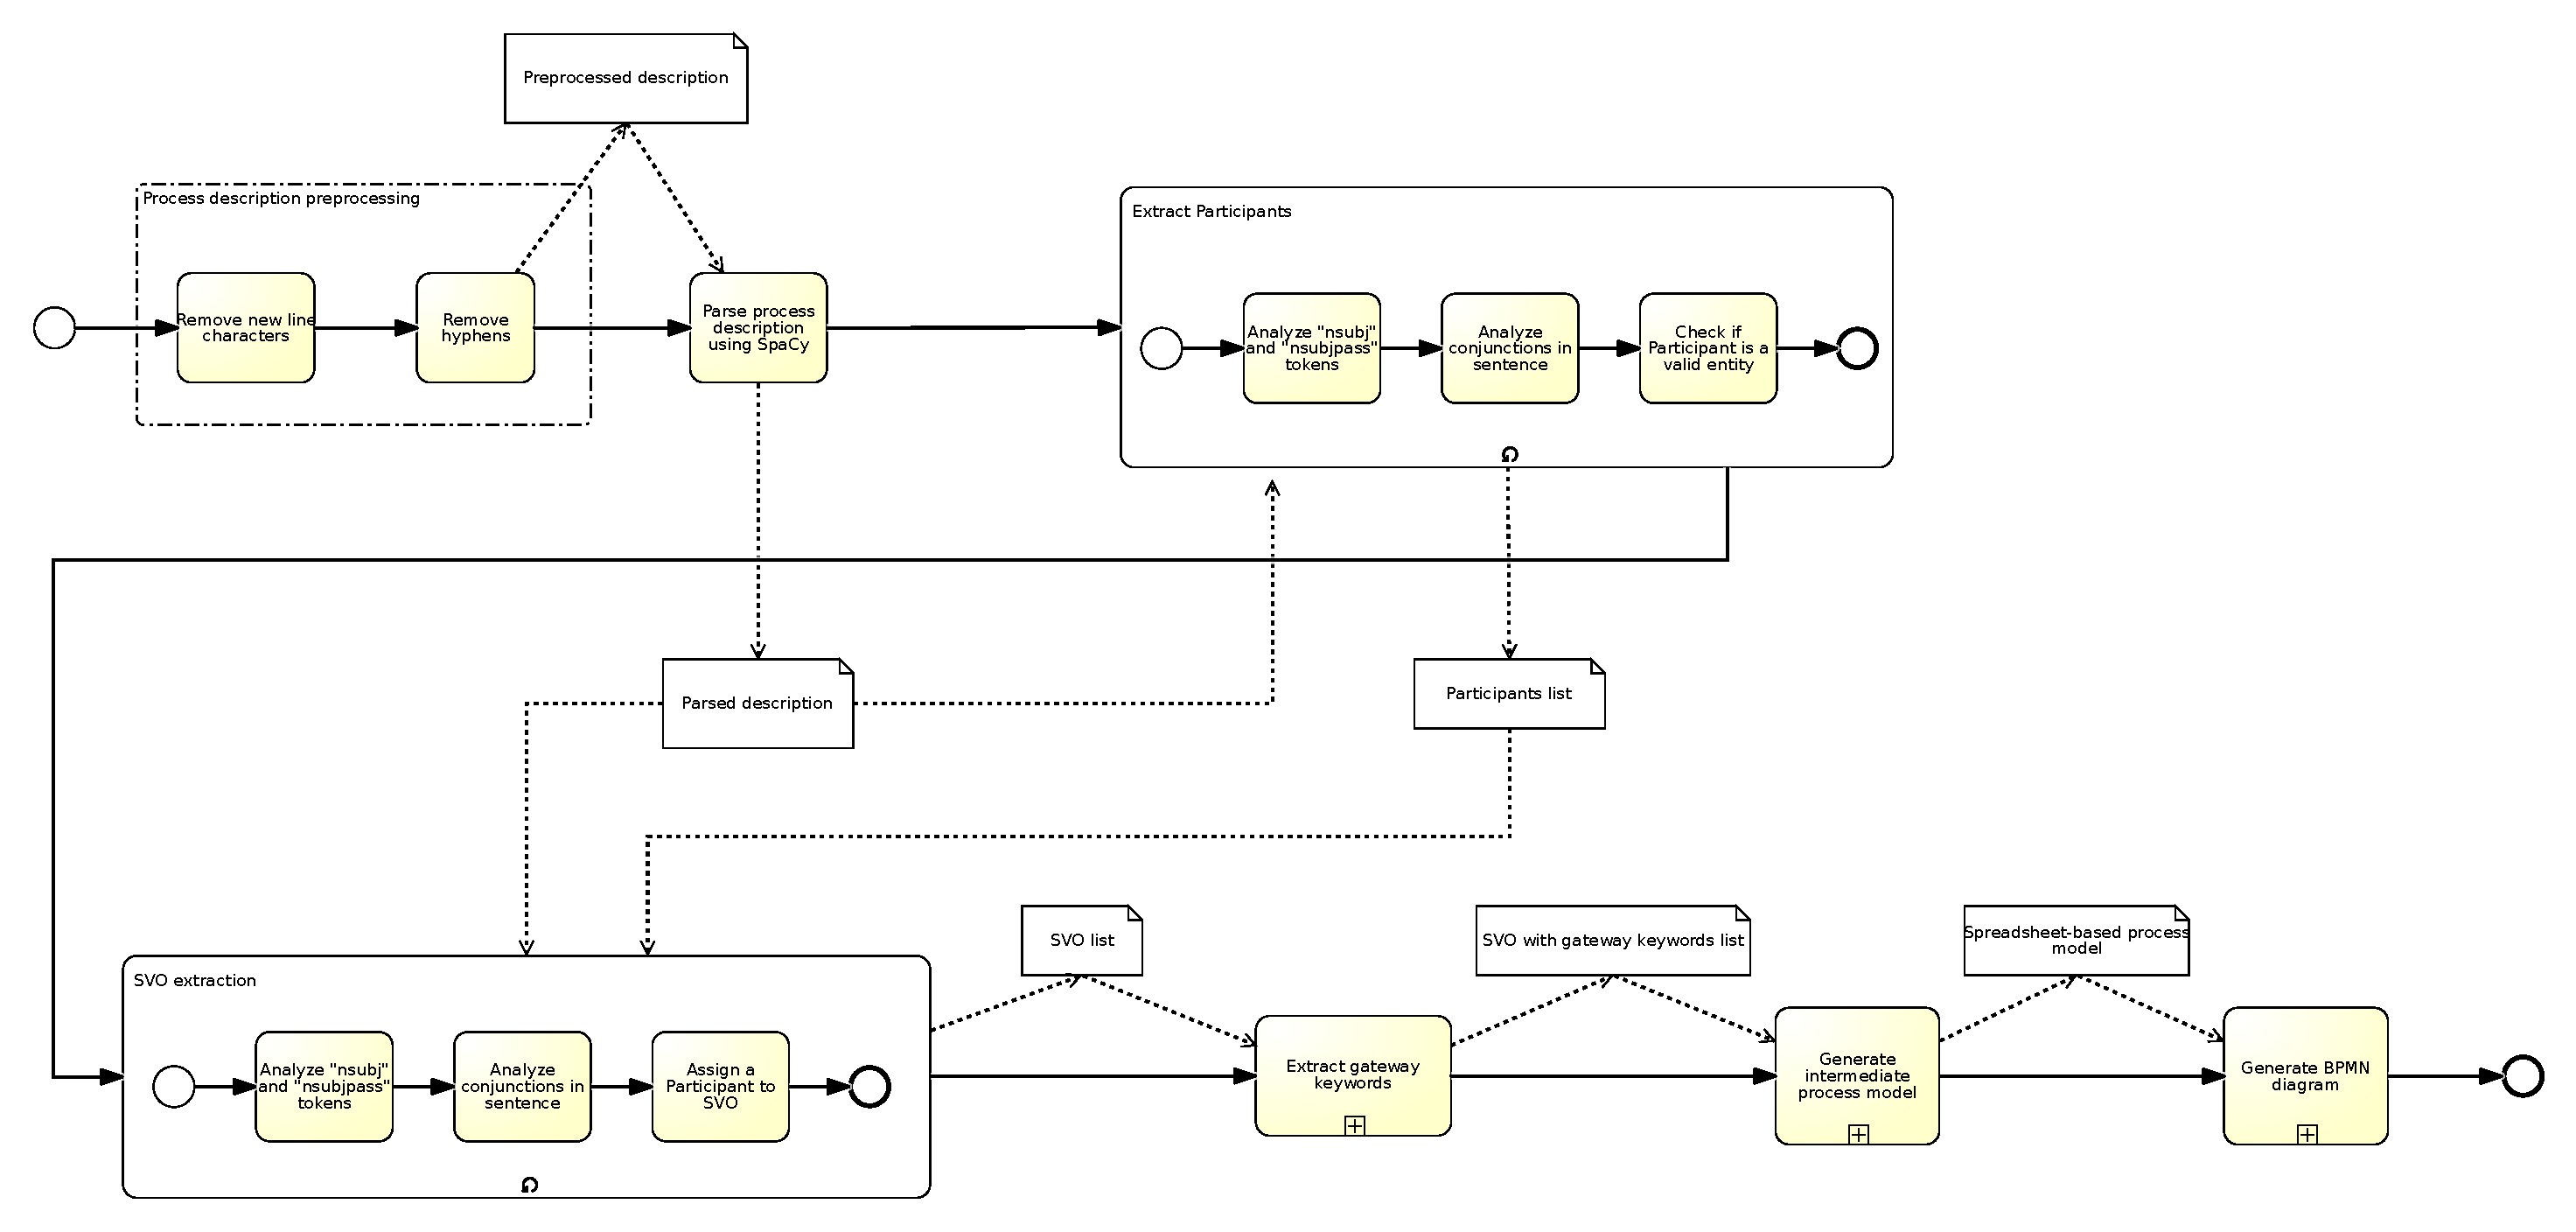
\includegraphics[width=0.95\textheight, angle=90]{./images/method_overview.pdf}
	\caption{BPMN diagram with overview of proposed approach.}
	\label{fig:method_overview}
\end{figure}

\section{Functional requirements}
The main functional requirement for the prototypical tool was portability of the created program. Thus, the prototype was implemented in Python language, since there are many implementations of Python interpreter, with official support for the most popular operating systems. In addition, many NLP processing tools (including SpaCy and WordNet) provide an API implemented in Python, thus Python is an interesting choice for many project from this field of computer science.\\
The tool was implemented using the newest, third version of Python language. This choice was made due to the fact, that third version provides a few new and interesting functionalities (such as built-in support for type annotation\footnote{\url{https://www.python.org/dev/peps/pep-0484/}, last access: \onlineAccess.}). Also, second version of Python language is officially considered as legacy version and no longer will be supported\footnote{\url{https://wiki.python.org/moin/Python2orPython3}, last access: \onlineAccess.}.\\
The prototypical tool works with SpaCy parser, version 1.6 -- this version was the newest one at the beginning of work.

\section{Participants extraction}
\label{sec:participant}
In the first step, each sentence of the description is analysed in search of words that represents participants in process. This process is divided into three parts.\\
First, the sentence is analysed in search of specific dependency relations, namely \emph{``nsub''} (nominal subject) and \emph{``nsubjpass''} (nominal subject passive). Whenever a token with one of these dependencies is found, it is added to the list of possible participants.\\
Next, the sentence is searched for conjunction (\emph{``conj''}) dependencies. In this case, the participant might be labelled as an object of the phrase. Therefore, the tokens belonging to the syntax sub-tree of conjunction is searched in order to find object-related dependency labels, that is \emph{``attr''} (attribute), \emph{``dobj''} (direct object), \emph{``iobj''} (indirect object) and \emph{``pobj''} (object of a preposition). For example, in the sentence: \emph{``It is given either by a sales representative or by a presales employee''} (syntax tree presented in Figure~\ref{fig:participant_conj_example}), the possible participant \emph{``employee''}, is labelled as object of preposition and word \emph{``by''} is labelled as a part of conjunction. Adding the conjunction check, it is possible to extract this information.\\
Figure~\ref{fig:participant_extraction_subprocess} shows BPMN diagram presenting overview of Particpant extraction algorithm.
\begin{figure}[H]
	\centering
	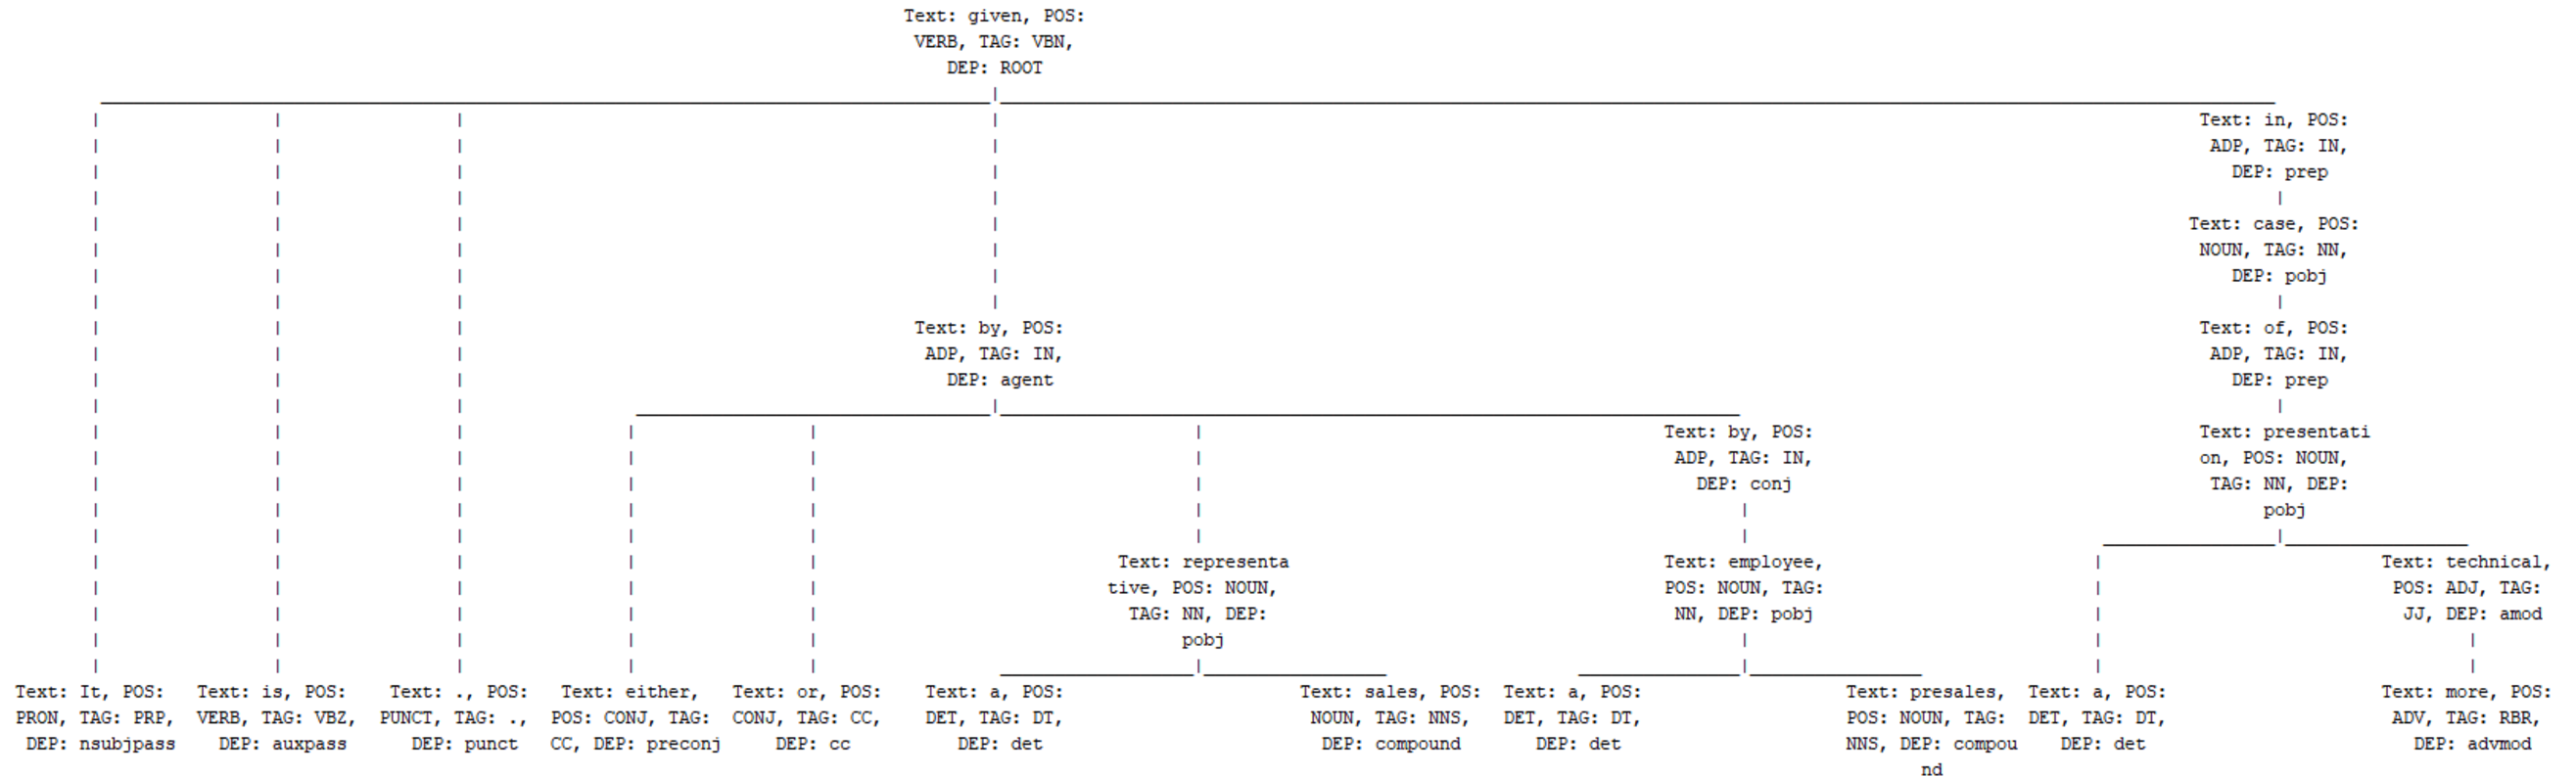
\includegraphics[width=\textwidth]{./images/participant_conj_example.pdf}
	\caption{Syntax tree for simple phrase \emph{``It is given either by a sales representative or by a presales employee in case of a more technical presentation.''} Word \emph{``employee''}, connected with conjunction dependency can be extracted as possible participant in business process.}
	\label{fig:participant_conj_example}
\end{figure}
\begin{figure}[H]
	\centering
	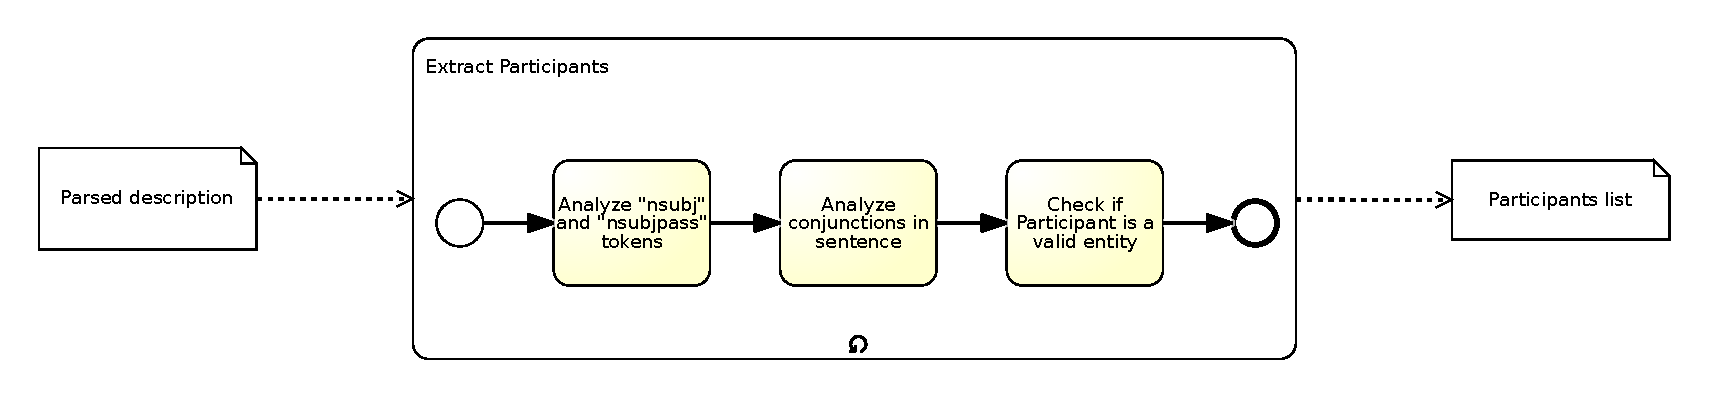
\includegraphics[width=\textwidth]{./images/participant_extraction_subprocess.pdf}
	\caption{BPMN diagram presenting overview of Particpant extraction algorithm}
	\label{fig:participant_extraction_subprocess}
\end{figure}
Every time, when a possible participant is added, its Part-Of-Speech tag -- based on Universal Dependencies tag set (mentioned in Section~\ref{subsec:syntax-parsing}) -- is checked. If the participant is tagged as a pronoun (\emph{pron}), a special flag is set for a given object.\\
Finally, a simple semantic analysis is used to decide, whether the extracted words can be used as participants of process. The extracted word is added to output as a participant if it fulfils one of these conditions:
\begin{itemize}
	\item the word is a pronoun or relative pronoun. In this case, the Participant is accepted as a valid entity,
	\item one of the hypernyms, derived from the analysed word, belongs to the specified list of hypernym keywords, accepted as participants. Examples of such keywords are \emph{``person''} or \emph{``organization''}. The full list of used hypernyms is shown in Table~\ref{table:participants-hypernyms}. Hypernyms of participant word are derived using WordNet lexical database,
	\item the word is equal to some special keyword. This case was added, because WordNet might not contain some specific words in the database, therefore hypernym analysis does not provide any proper result. An example could be the word CRM (Customer Relationship Management). A full list of keywords used in this prototype is shown in Table~\ref{table:participants-keywords}. List was composed through analysis of test set of process descriptions.
\end{itemize}	
Each of the Participants have a full name assigned, which is extracted from its syntax sub-tree, provided that a given token from sub-tree is labelled with a correct dependency. In case of Participant, the following dependencies are used in full name (definitions of these dependencies are shown in Table~\ref{table:dependencies}):
\begin{itemize}
	\item amod, 
	\item acomp, 
	\item aux,
	\item auxpass,
	\item compound,
	\item neg,
	\item poss.
\end{itemize}
An example spreadsheet-based model, extracted from the sentence: \emph{``Whenever the sales department receives an order, a new process instance is created.''} (syntax tree presented in Figure~\ref{fig:participant_example}), is shown in Table~\ref{csv:participant_example}. In compliance to the described approach, two possible participants are extracted: \emph{``department''} (tagged with dependency \emph{``nsubj''}) and \emph{``instance''} (tagged with dependency \emph{``nsubjpass''}). During the semantic analysis phase, the word \emph{``instance''} is discarded, as it does not have hypernym associated with the accepted set of hypernyms. Thus, only the word \emph{``department''} is accepted as participant. In the generated intermediate model, the activity \emph{``Receive An Order''} has a participant \emph{``Sales Department''} (this is the full name of the \emph{``department''} participant, extracted from a given sentence) added in \emph{``Who''} column. The second activity \emph{``Create Process Instance''}, does not have information about participant, since it was discarded earlier.
\begin{figure}[H]
	\centering
	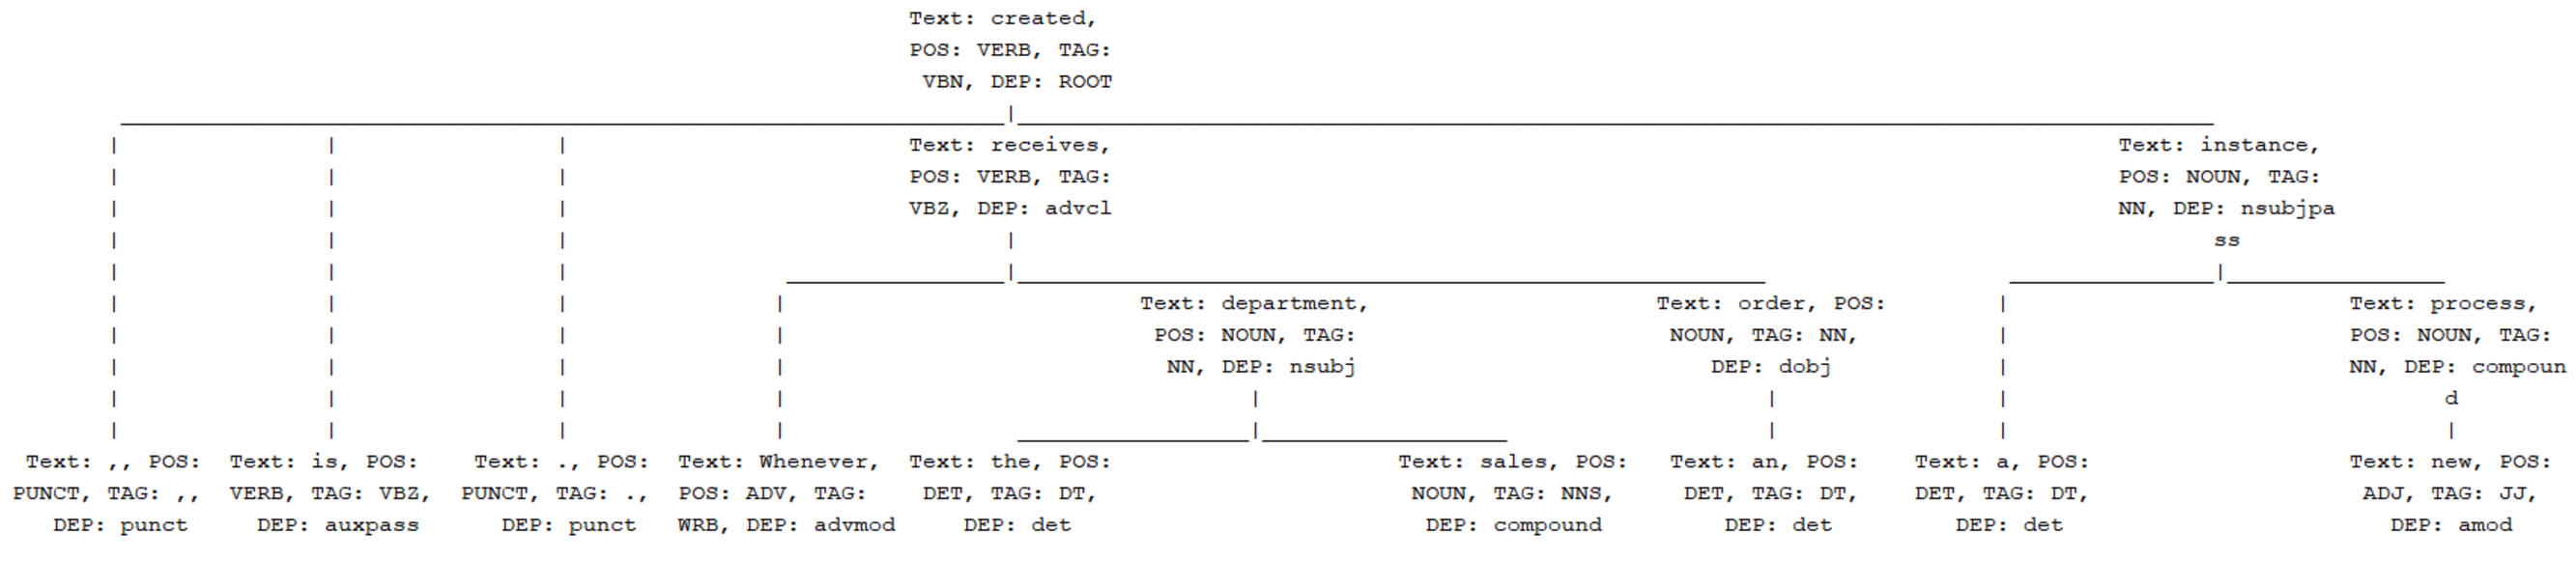
\includegraphics[width=\textwidth]{./images/participant_example.pdf}
	\caption{A syntax tree for the simple phrase \emph{``Whenever the sales department receives an order, a new process instance is created.''}}
	\label{fig:participant_example}
\end{figure}
{\scriptsize
\begin{longtable}{|p{0.03 \hsize}|p{0.25 \hsize}|p{0.15 \hsize}|p{0.2 \hsize}|p{0.1 \hsize}|p{0.1 \hsize}|}
	\hline
	Order & Activity & Condition & Who & Subprocess & Terminated.
	\\\hline\hline
	\csvreader[late after line=\\\hline]
	{./results/participant_example.csv}
	{Order=\Order,Activity=\Activity,Condition=\Condition,Who=\Who,Subprocess=\Subprocess,Terminated=\Terminated}
	{\Order & \Activity & \Condition & \Who & \Subprocess & \Terminated}
	\caption{Spreadsheet-based description generated from the sentence: \emph{``Whenever the sales department receives an order, a new process instance is created.''}}
	\label{csv:participant_example}
\end{longtable}
}
Listing~\ref{lst:participant_extraction} presents a Python script with the participant extraction implementation.\\
\lstinputlisting[language=Python, caption={Participant extraction function listing}, label={lst:participant_extraction}]{./listings/extract_participants.py}

\section{Subject-Verb-Object extraction}
\label{sec:svo}
After extracting the participants from the sentence, syntactic analysis in search of SVO (subject-verb-object) constructs is performed. These construct are used to generate intermediate process model.\\
First, the sentence is searched for \emph{``nsubj''} and \emph{``nsubjpass''} dependencies. For every word found, a new SVO construct is added to the output. In the case of words with nominal subject dependency, the subject is created from the extracted word, its predecessor in the syntax tree acts as a verb and the object is extracted from the subject's ancestors in syntax tree. The search for the object is divided into two phases.\\
First, a shallow search -- in which case only direct ancestors (children) in syntax sub-tree are analysed in search for tokens with two dependencies: \emph{``attr''} (attribute), \emph{``dobj''} (direct object). If object was not found during shallow search, a deep search (which involves all of the ancestors) with larger dependencies set -- \emph{``dobj''} (direct object), \emph{``iobj''} (indirect object), \emph{``pobj''} (object of preposition), \emph{``attr''} (attribute), \emph{``xcomp''} (open clausal complement). If the appropriate token is found, it is added as an object to SVO, otherwise the object part of SVO construct is omitted. Separating the object search into two phases improves the extraction results -- in most cases, the object is directly connected to the verb by \emph{``attr''} and \emph{``dobj''} dependency.  In case of tokens with nominal subject passive dependency, the object is omitted. For example, in the  sentence: \emph{``Purchase is registered''}, the word \emph{``Purchase''} is tagged as \emph{``nsubjpass''} and no object is present.\\
Similarly to the participants extraction, the SVO extraction also analyses the existence of conjunction in sentences. After finding a conjunction and validation its POS tag (this way, the conjunction which are not verbs are eliminated), it is used as a verb for a new SVO construct and the object is extracted from its children. Then, the syntax tree is analysed in search of the subject of a new construct. If the subject is found, a new SVO is created. This approach helps to deal with the sentences like: \emph{``If the storehouse has successfully reserved or backordered every item''}. In this case, by conjunction analysis it is possible to extract construct \emph{``backordered every item''}, which is conjoined by word \emph{``backordered''}.\\
In the last step, the extracted SVOs are connected with the corresponding participants, which were discovered by previous function in this sentence. Attaching participant to SVO will provide additional information during intermediate process model generation.\\
Figure~\ref{fig:svo_extraction_subprocess} shows BPMN diagram presenting overview of SVO extraction algorithm.
\begin{figure}[H]
	\centering
	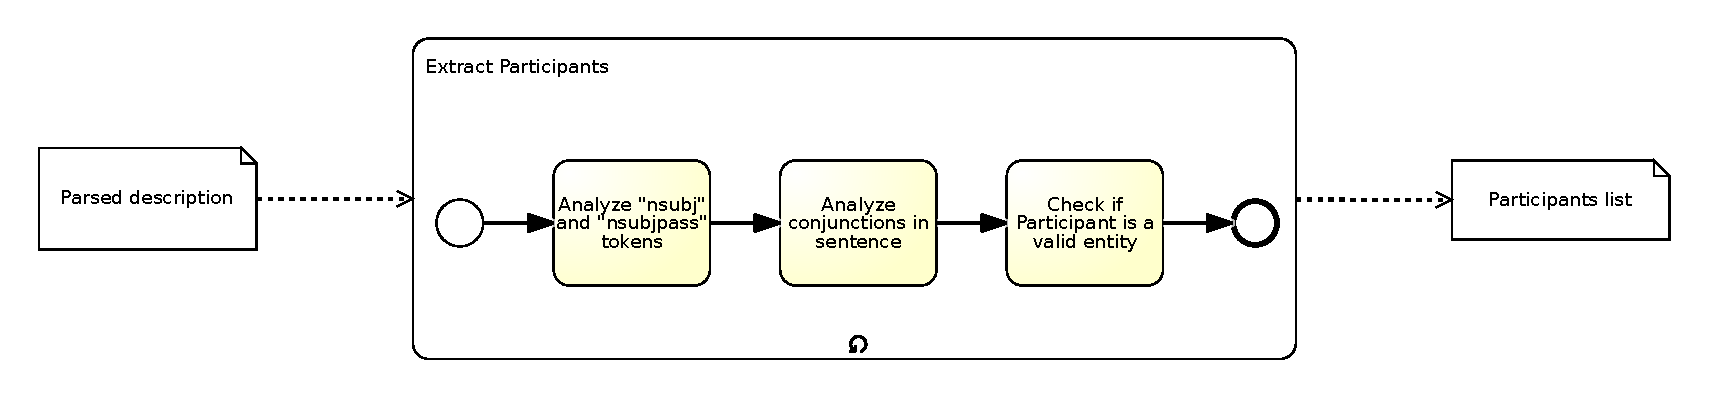
\includegraphics[width=\textwidth]{./images/participant_extraction_subprocess.pdf}
	\caption{BPMN diagram presenting overview of SVO extraction algorithm}
	\label{fig:svo_extraction_subprocess}
\end{figure}
Similarly to Participants, the SVOs have also a full name assigned. The difference lies in the accepted list of dependency labels. For the SVO, the following dependencies are used in full name (definitions of these dependencies are shown in Table~\ref{table:dependencies}):
\begin{itemize}
	\item amod, 
	\item acomp, 
	\item aux,
	\item auxpass,
	\item neg.
\end{itemize}
An example of SVO extraction is shown in Table~\ref{csv:svo_example}. In this case, a~simple sentence \emph{``Afterwards, the sales department ships the bicycle to the customer and finishes the process instance''} was processed. Two SVO constructs were extracted: \emph{``Sales Department ships bicycle''} and \emph{``Sales Department finishes process instance''}. The \emph{``Sales Department finishes process instance''} SVO was extracted using conjunction dependency, since the token \emph{``finishes''} is tagged with \emph{``conj''} dependency. In both cases, an appropriate participant (\emph{Sales Department}) was attached to activity and added to generated spreadsheet.
\begin{figure}[H]
	\centering
	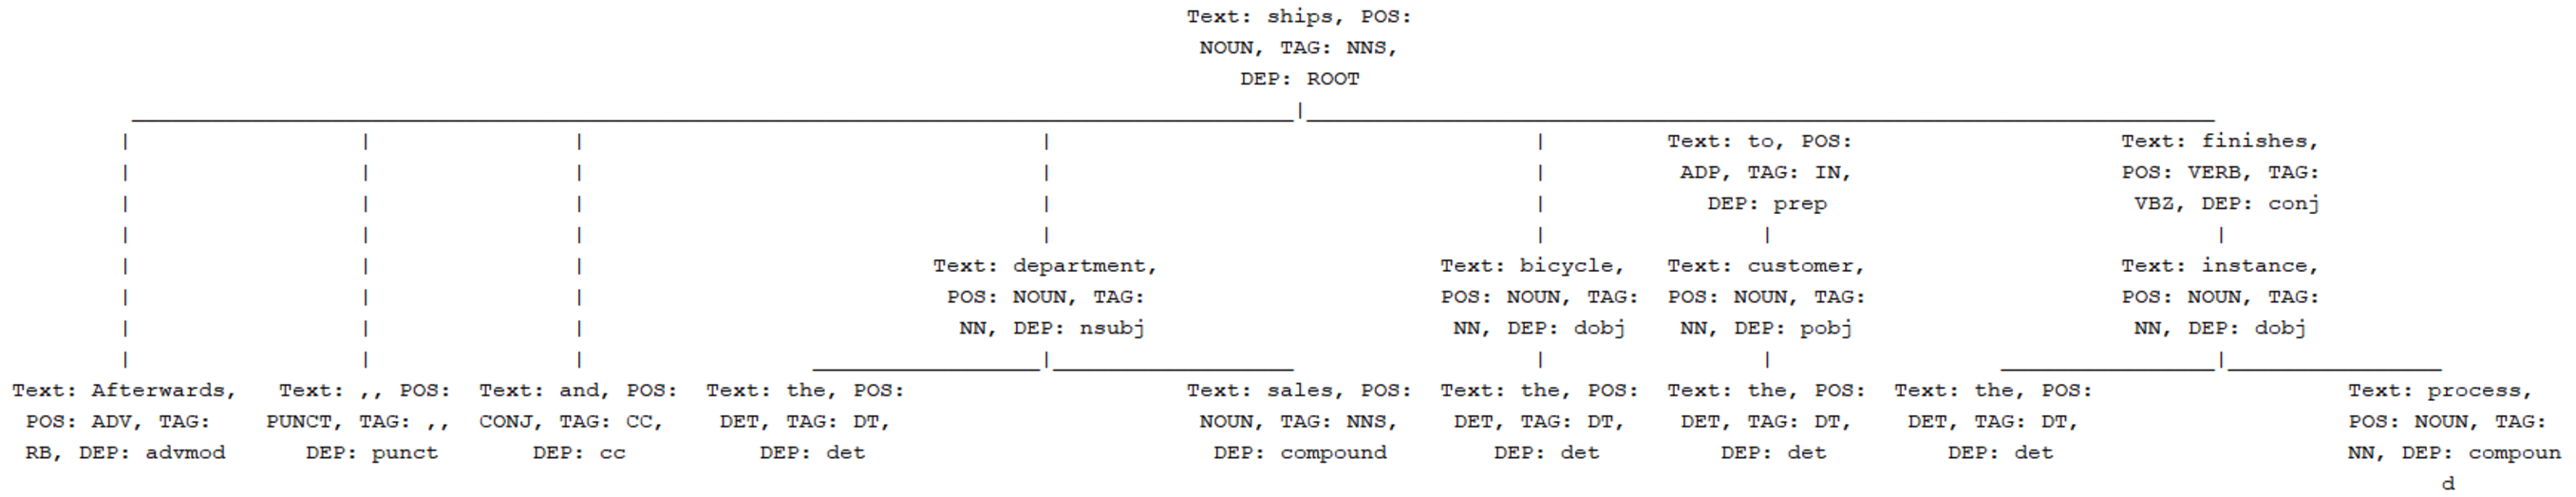
\includegraphics[width=\textwidth]{./images/svo_extraction_example.pdf}
	\caption{Syntax tree for simple phrase \emph{``Afterwards, the sales department ships the bicycle to the customer and finishes the process instance''}}
	\label{fig:svo_example}
\end{figure}
{\scriptsize
	\begin{longtable}{|p{0.03 \hsize}|p{0.25 \hsize}|p{0.15 \hsize}|p{0.2 \hsize}|p{0.1 \hsize}|p{0.1 \hsize}|}
		\hline
		Order & Activity & Condition & Who & Subprocess & Terminated.
		\\\hline\hline
		\csvreader[late after line=\\\hline]
		{./results/svo_extraction_example.csv}
		{Order=\Order,Activity=\Activity,Condition=\Condition,Who=\Who,Subprocess=\Subprocess,Terminated=\Terminated}
		{\Order & \Activity & \Condition & \Who & \Subprocess & \Terminated}
		\caption{Spreadsheet-based description generated from sentence: \emph{``Afterwards, the sales department ships the bicycle to the customer and finishes the process instance''}}
		\label{csv:svo_example}
	\end{longtable}
}
Listing~\ref{lst:svo_extraction} presents a Python script with SVO extraction implementation.\\
\lstinputlisting[language=Python, caption={Subject-Verb-Object extraction function listing}, label={lst:svo_extraction}]{./listings/extract_svo_constructs.py}

\section{Gateway keywords search}
After extracting the participants and subject-verb-object constructs, the whole description is analysed once more, in order to find keywords which indicate the existence of possible gateway. This function searches for three different types of keywords: conditional, parallel and default flow. The first type can be later translated either into an exclusive gateway or into an inclusive gateway, second -- into a parallel gateway. Third type might be used as a default flow of conditional gateway, provided that the correspondence with a conditional keyword will be found during model generation. If no correspondence is found, the SVO will be treated as a simple activity. The list of keywords are shown in Table~\ref{table:gateway-keywords}.\\
This function simply performs a word-by-word search of keywords. After finding one, the syntax tree is analysed in search of token which belongs to the SVO construct and which verb is a predecessor of keyword token that was found.\\
An example of conditional flow extracted from process description is shown in Table~\ref{csv:gateway_example}. A sentence \emph{``If the customer decides that the costs are acceptable, the process continues, otherwise she takes her computer home unrepaired.''} from the process description~\ref{txt:gateway_example} is translated into two activities, which are parts of conditional flow. Because the keyword associated with default flow was found and and activity with condition \emph{``else''} was added, a XOR gateway was added to the diagram.
\begin{tcolorbox}[
	breakable,
	arc=0mm,
	left=1pt,
	right = 1pt,
	boxrule=0mm,
	colback = {white},
	]
	\texttt{\input{./models/gateway_example.txt}}
\end{tcolorbox}
\captionof{textdesc}{Fragment of a process description with extractable conditional gateway}
\label{txt:gateway_example}
{\scriptsize
	\begin{longtable}{|p{0.03 \hsize}|p{0.20 \hsize}|p{0.15 \hsize}|p{0.1 \hsize}|p{0.1 \hsize}|p{0.1 \hsize}|}
		\hline
		Order & Activity & Condition & Who & Subprocess & Terminated.
		\\\hline\hline
		\csvreader[late after line=\\\hline]
		{./results/gateway_example.csv}
		{Order=\Order,Activity=\Activity,Condition=\Condition,Who=\Who,Subprocess=\Subprocess,Terminated=\Terminated}
		{\Order & \Activity & \Condition & \Who & \Subprocess & \Terminated}
		\caption{Spreadsheet-based description generated from a text description shown in Text~\ref{txt:gateway_example}}
		\label{csv:gateway_example}
	\end{longtable}
}
\begin{figure}[H]
	\centering
	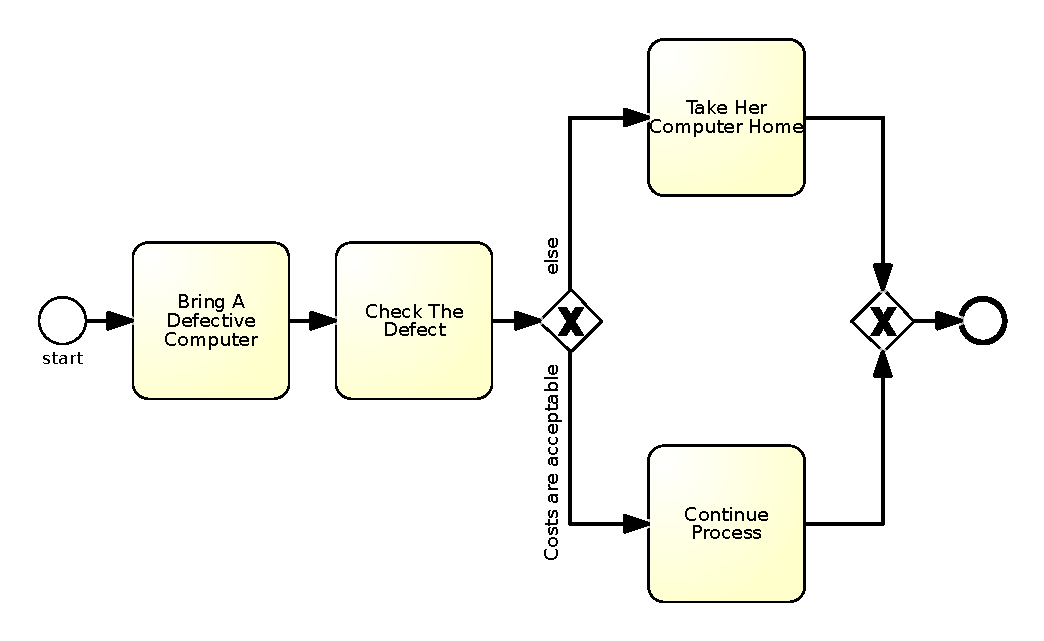
\includegraphics[scale=0.55]{./images/gateway_example.pdf}
	\caption{BPMN diagram with an XOR gateway, generated from the intermediate process model shown in Table~\ref{csv:gateway_example}}
	\label{fig:gateway_example}
\end{figure}
The Listing~\ref{lst:gateway_extraction} presents a Python script with gateway keywords extraction implementation.
\lstinputlisting[language=Python, caption={Gateway keywords search function listing}, label={lst:gateway_extraction}]{./listings/find_gateway_keywords.py}

\section{Prototype model generation}

\subsection{Intermediate model description}
The prototype implementation uses a spreadsheet-based process description, which employs a CSV (Comma-Separated Values) file format to represent a business process model. This spreadsheet-based process description is presented in the article~\cite{kluza-spreadsheet}. A business process is described by a spreadsheet table. Each row represents a single phase, which can be translated into a BPMN task or sub-process. Columns represent the properties of each phase. Overall, there are six properties:
\begin{itemize}
	\item Order -- number of the corresponding phase. Parallel or excluding tasks are distinguished by suffix created from the consecutive letters (a-z). In the case of nested gateways, another suffix, with number of phase and letter for branch is added. Table~\ref{csv:csv_order_example} shows an example of spreadsheet-based process model. Notice that activities \emph{``Initiate search''} and \emph{``Track files''} are parts of conditional flow, thus the order number has a branch suffix added,
	
	{\scriptsize
		\begin{longtable}{|p{0.03 \hsize}|p{0.25 \hsize}|p{0.15 \hsize}|p{0.2 \hsize}|p{0.1 \hsize}|p{0.1 \hsize}|}
			\hline
			Order & Activity & Condition & Who & Subprocess & Terminated.
			\\\hline\hline
			\csvreader[late after line=\\\hline]
			{./results/csv_order_example.csv}
			{Order=\Order,Activity=\Activity,Condition=\Condition,Who=\Who,Subprocess=\Subprocess,Terminated=\Terminated}
			{\Order & \Activity & \Condition & \Who & \Subprocess & \Terminated}
			\caption{Spreadsheet-based description generated from sentence: \emph{``Afterwards, the sales department ships the bicycle to the customer and finishes the process instance''}}
			\label{csv:csv_order_example}
		\end{longtable}
	}

	\item Activity -- name of the performed action. There is a special case -- \emph{``goto X''} is a special statement, which signalizes that a part of the process must be skipped or there is a loop in a process. Table~\ref{csv:activity_csv_example} shows an example of spreadsheet-based process model. Notice the special statement \emph{``goto 5''} in activity \emph{4b1},
	
	{\scriptsize
		\begin{longtable}{|p{0.03 \hsize}|p{0.25 \hsize}|p{0.15 \hsize}|p{0.2 \hsize}|p{0.1 \hsize}|p{0.1 \hsize}|}
			\hline
			Order & Activity & Condition & Who & Subprocess & Terminated.
			\\\hline\hline
			\csvreader[late after line=\\\hline]
			{./results/csv_activities_example.csv}
			{Order=\Order,Activity=\Activity,Condition=\Condition,Who=\Who,Subprocess=\Subprocess,Terminated=\Terminated}
			{\Order & \Activity & \Condition & \Who & \Subprocess & \Terminated}
			\caption{An example of spreadsheet-based process model with multiple activities}
			\label{csv:activity_csv_example}
		\end{longtable}
	}
	
	\item Condition -- a condition, which has to be fulfilled in order to perform the task. This property is used to implement the exclusive and inclusive gateway. In the first case, a gateways should consist of at least two tasks, one of which should be filled with condition. The last one from all of the tasks that belong to the gateway should contain a keyword \emph{``else''} as a condition. In case of inclusive gateway, both tasks should contain the corresponding conditions. Table~\ref{csv:gateway_csv_example} shows an example of spreadsheet-based process model with conditional flow included. In this case, activities \emph{``Approve Loan''} and \emph{``Deny Loan''} will be connected by inclusive gateway, since both activities have a condition and there is not \emph{``else''} keyword,
	
	{\scriptsize
		\begin{longtable}{|p{0.03 \hsize}|p{0.20 \hsize}|p{0.15 \hsize}|p{0.1 \hsize}|p{0.1 \hsize}|p{0.1 \hsize}|}
			\hline
			Order & Activity & Condition & Who & Subprocess & Terminated.
			\\\hline\hline
			\csvreader[late after line=\\\hline]
			{./results/csv_condition_example.csv}
			{Order=\Order,Activity=\Activity,Condition=\Condition,Who=\Who,Subprocess=\Subprocess,Terminated=\Terminated}
			{\Order & \Activity & \Condition & \Who & \Subprocess & \Terminated}
			\caption{Spreadsheet-based description with conditional flow included}
			\label{csv:gateway_csv_example}
		\end{longtable}
	}
	
	\item Who – the name of person, system or department responsible for executing this phase. This property can be transformed into a swimlane in BPMN diagram,
	\item Subprocess -- this property informs that a task should be considered as a sub-process. This column should be filled with \emph{``yes''} (if the task is a sub-process), or left empty otherwise,
	\item Terminated -- this property informs that a given task terminates the process. This column should be filled with \emph{``yes''} if this is the case.
\end{itemize}
The spreadsheet-based process description presented in article~\cite{kluza-spreadsheet} supports only basic BPMN elements. However, the subset of supported BPMN elements covers the most commonly used elements of BPMN diagram~\cite{bpmn-stats}. Moreover, the supported subset covers all of the elements required for the purpose of this thesis as well.
\begin{figure}
	\centering
	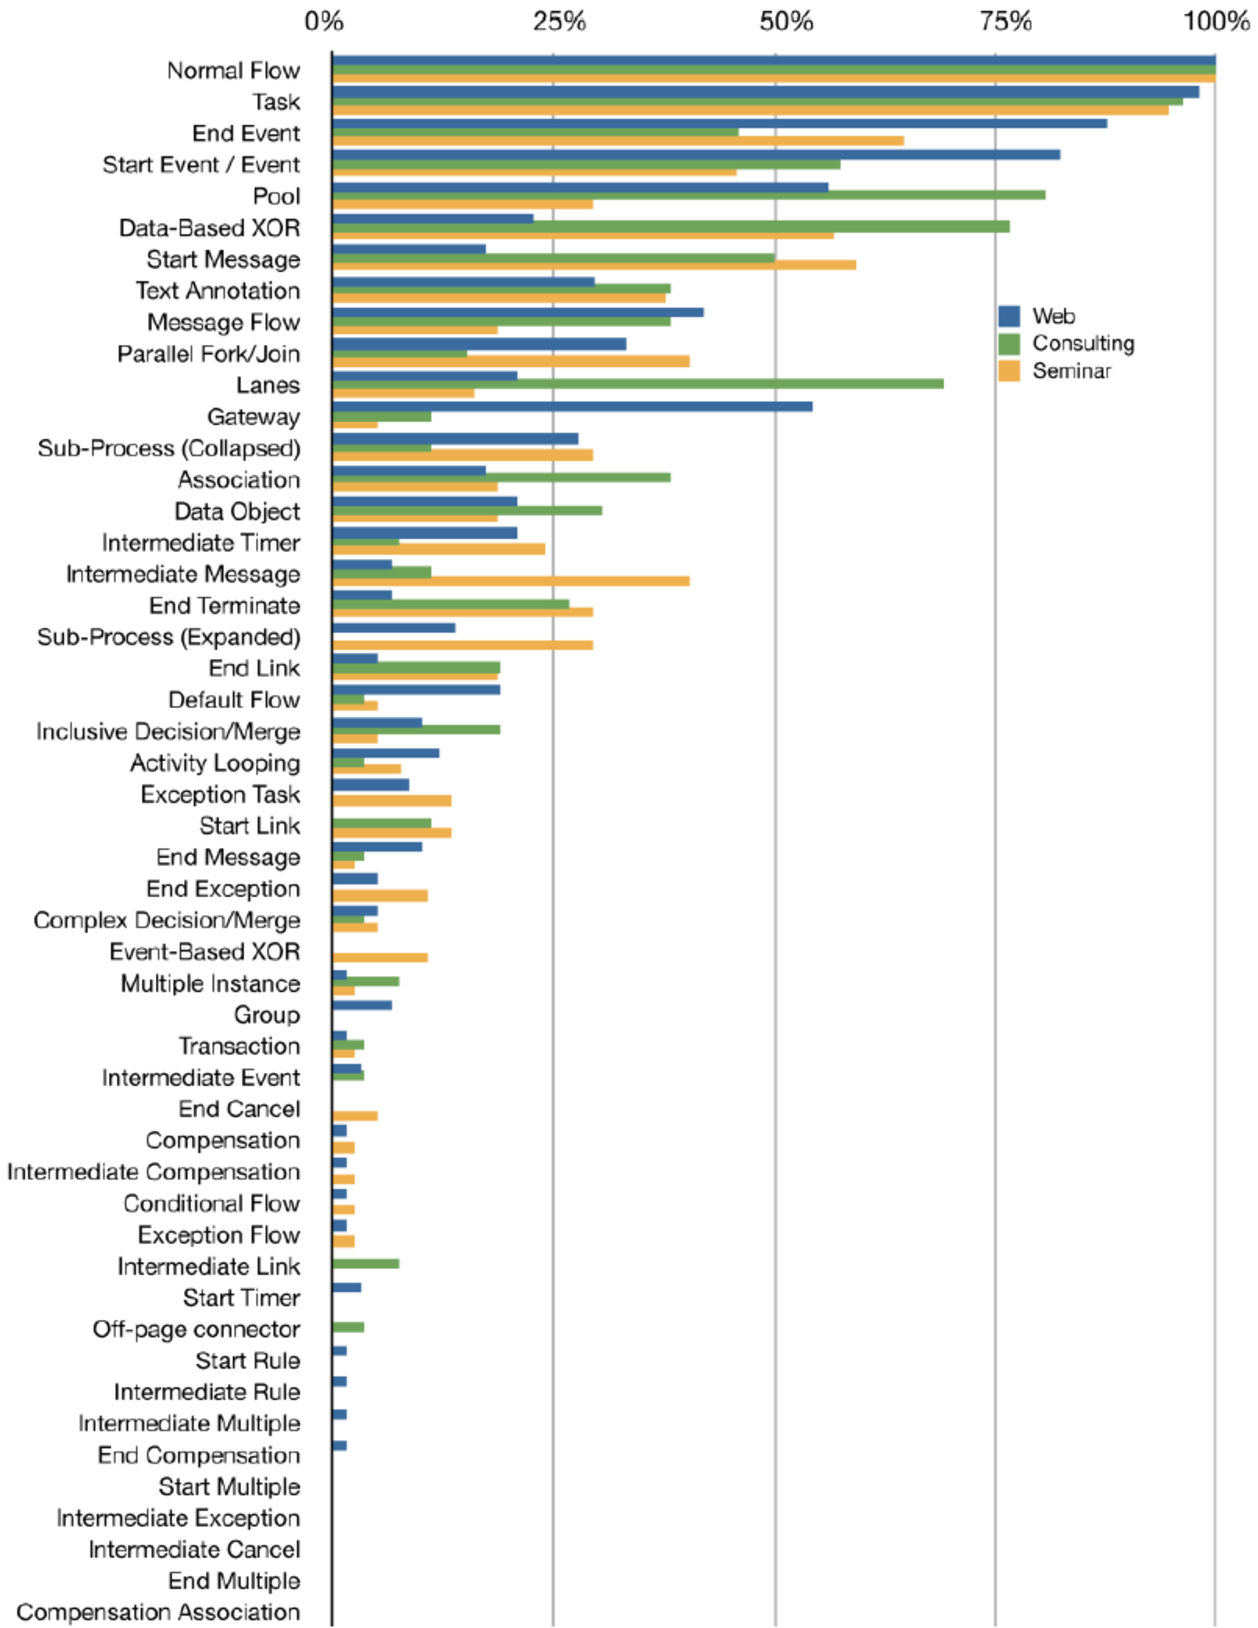
\includegraphics[width=\textwidth]{./images/bpmn_usage_stats.pdf}
	\caption{Frequency of occurrence diagram for BPMN elements. Diagram obtained from article~\cite{bpmn-stats}}
	\label{fig:bpmn_usage_stats}
\end{figure}

\subsection{Spreadsheet-based model generation approach}
The final part of the implemented prototype is the intermediate process model generation phase. This phase makes use of previous functions to discover information useful for process model. As it was said earlier, the final product of this phase is a spreadsheet-based model, which is used to generate BPMN diagram and can be revised by a human expert.\\
Before the extraction process begins, a simple text preprocessing is performed. It basically consists of two actions:
\begin{itemize}
	\item removing all newlines and replacing them with whitespaces,
	\item removing hyphens from the description.
\end{itemize}
Both of these steps are performed in order to fix some of the parser issues. The presence of newline characters (\emph{``\texttt{\textbackslash n}''} used in operating systems based on Unix core and \emph{``\texttt{\textbackslash r\textbackslash n}''} in operating systems from Windows family) results in the situation where sentences are incorrectly split -- newline is treated as a~single, empty sentence, and it breaks the sentences into two unrelated pieces. Removal of hyphens is performed in order to fix the issue with compound verbs and adjectives (such as "pre-sales"). Compounds are split into multiple words during syntax parsing, which makes the extraction of Participant or SVO full name difficult -- some of the information may be lost.\\
In the first phase, the elements (participants and SVO) extraction is performed. Next, the gateway keywords search proceeds. After these initial steps, the list of process activities is initialized -- start activity is inserted. Next, the Subject-Verb-Object constructs are sorted by their chronological appearance in the text. After that, the program iterates over a list of extracted SVO. For each construct, the appropriate action, based on a set of conditions, should be performed:
\begin{itemize}
	\item if the SVO is labelled with a conditional gateway keyword, it is added to the intermediate model as a part of conditional gateway. If there was a parallel gateway detected earlier, the appropriate flag is set to false. Next, the conditional gateway is initialized by setting up the conditional gateway flag and helper variables. The usage of gateway flag helps to deal with sentences such as \emph{``If <first condition>, <action>. If <second condition>, <action>''} which should be treated as a parts of single gateway. After the initialization, current SVO and next one from the list are added to the model as a condition-action of a conditional gateway. This part works under the assumption, that the condition (also extracted as a SVO) is mentioned before action. In compliance to the intermediate model requirements, the property \emph{``Condition''} is filled with a full name of the condition SVO. If the condition SVO has a participant attached and it is not a pronoun, the full name of participant is entered as the \emph{``Who''} property. Otherwise, it is left empty,
	\item SVO labelled with a parallel gateway keyword is treated in a similar way. The main difference is that after initialization, the next SVO from a list is added as a parallel task to the current SVO. This approach should work with simple sentences, such as \emph{``while <action one>, <action two>''}, in which the parallel tasks are mentioned consecutively. Similarly to the conditional gateway rule, if the inserted actions has a participant attached and it is not a pronoun, the \emph{``Who''} property is filled with its full name or left empty otherwise,
	\item if the SVO is labelled as default flow, the behaviour of function depends on previously detected gateways. If the parallel gateway was found, the SVO is added as another task in this gateway. For the conditional gateway, a default flow is added -- an additional task, with keyword \emph{``else''} entered as a \emph{``Condition''} property. A default flow is recognized by the keyword \emph{``else''} in condition column. If none of the gateways were added previously, the SVO is added as a simple task. This option was added, so that the potentially useful information would not be lost. The SVO will be added as a task, provided that it has a validated participant attached. This is performed in order to filter out the unnecessary SVO, which should not be treated as tasks, but only provides some information about conditions in gateways or other descriptive information. In all of these cases, the participant attached to the action is treated exactly like in previous options,
	\item if none of the previous options were executed, the SVO is added as a simple task, connected by a sequence flow. Before a new task is added, gateway flags are checked. In the case of parallel gateway flag, it is set to false. In case of the conditional gateway flag, a gateway branch index is evaluated. If it is lower that two, a default flow (activity with \emph{``Condition''} set to \emph{``else''}), which points to the end event (which is achieved by naming the activity as \emph{``goto X''}, where X is a current value of order, incremented by one), is added to the gateway. This is performed due to the fact, that the conditional gateway with one conditional flow, will result in deadlock -- if the only condition is false, the process cannot be continued. After this check, the SVO construct can be added as a~simple task. The participant attached is handled similarly like in previous situations.
\end{itemize}
Figure~\ref{fig:intermediate_model_generation} shows the BPMN diagram presenting overview of intermediate process model description generation algorithm.\\
\begin{figure}
	\centering
	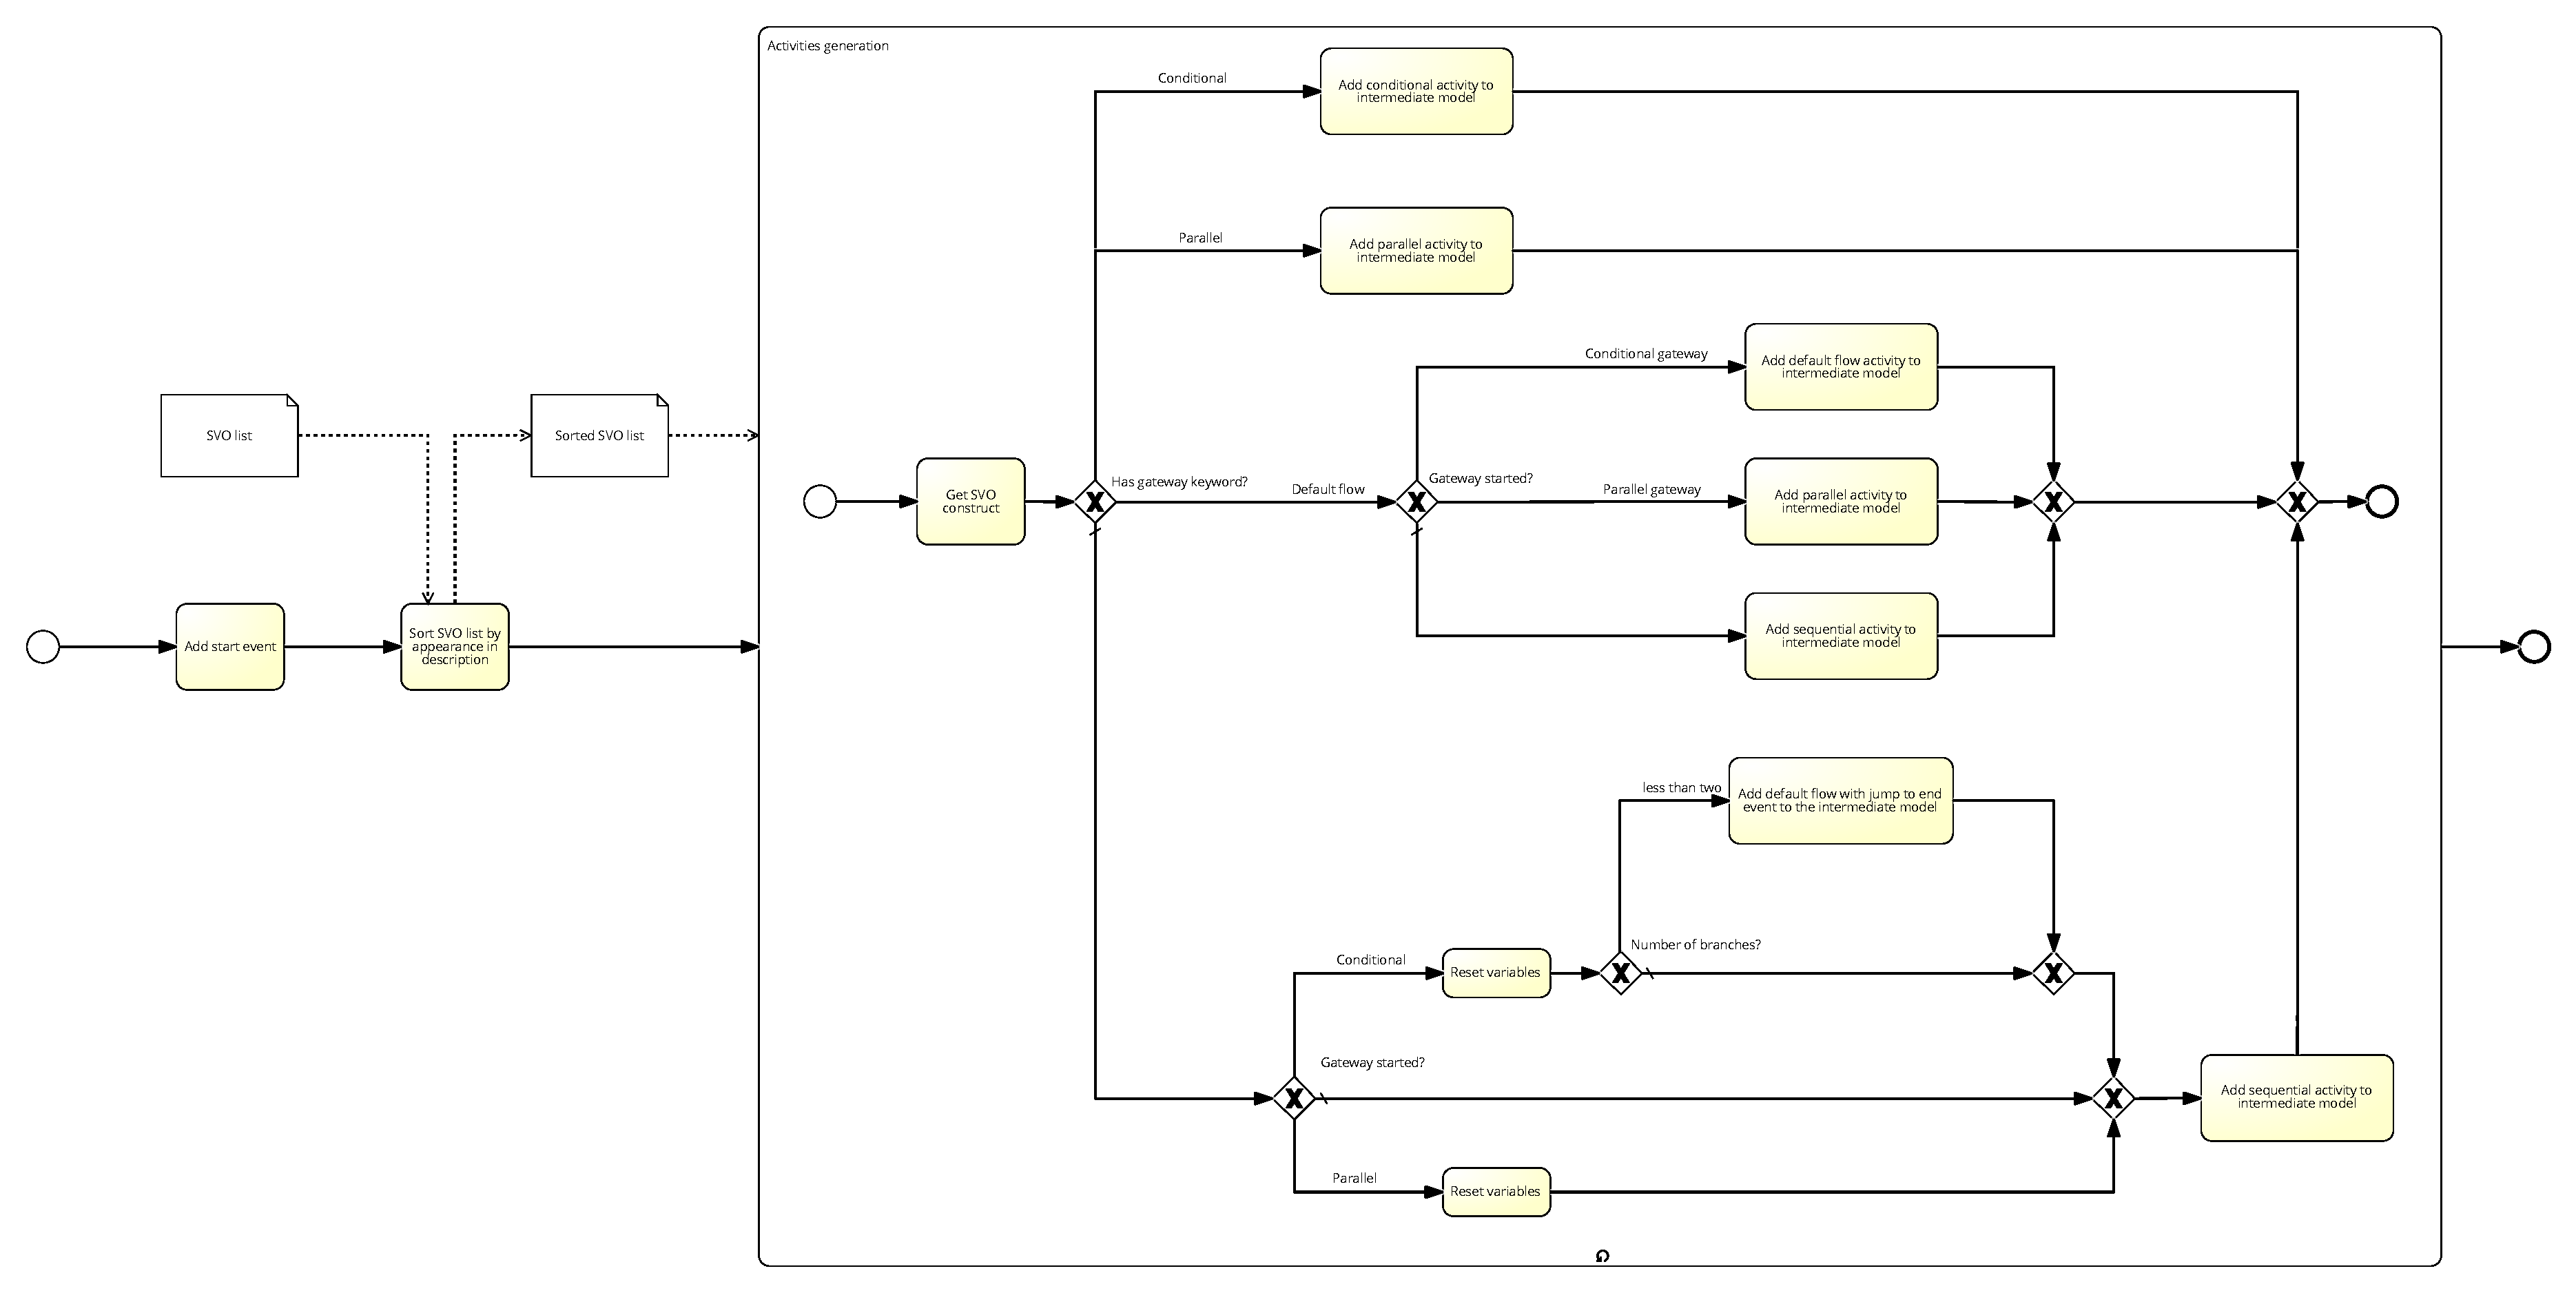
\includegraphics[width=0.95\textheight, angle=90]{./images/intermediate_model_generation.pdf}
	\caption{BPMN diagram presenting overview of intermediate process model description generation algorithm}
	\label{fig:intermediate_model_generation}
\end{figure}
After all of the subject-verb-objects constructs are processed, the conditional gateway flag is validated once more -- similarly to the last case, if conditional gateway has only one conditional flow, a default flow is added. Finally, the end event is added, which finishes the intermediate process generation.\\
Before a new activity is added to the intermediate model, the SVO which serves as a basis for the activity is validated. Validation process checks if the base form of verb part of SVO belongs to one of two sets of specific verbs. The first set is called \emph{``ignorable verbs''} and consists of verbs such as \emph{``need''}, \emph{``exist''}. Using this set, it is possible to discard SVO that clearly should not be converted into activity, since these SVO does not provide any information about the activity. An example of such SVO is \emph{``Customer does not exist''} which does not indicate any activity that should be performed -- this SVO might rather be used as a condition. The second set, called \emph{``replaceable verbs''} contains verbs like \emph{``be''} or \emph{``do''}. These verbs indicate that SVO might contain information about possible activity, but the correct verb should be found. The search is performed by checking the verb token syntax sub-tree in search of token tagged with \emph{VERB} POS tag, which is neither ignorable or replaceable verb. An example of SVO which includes the replaceable verb, but can be converted into activity can be phrase \emph{``Patient is examined''}. This SVO can be converted into valid activity \emph{``Examine Patient''}. An example of SVO which includes the replaceable verb, but do not provide information about activity, can be phrase \emph{``Part is available''}. This SVO could be used as a condition of the gateway, but is not a valid activity.\\
After checking if SVO should be converted into an activity, the conversion process begins. First, it is decided whether activity should be ordered as Verb-Subject or Verb-Object. If the object is missing from SVO or it is tagged as \emph{VERB}, the former is chosen. Otherwise, the Verb-Object form is chosen. This allows to distinct between phrases such as \emph{``Process instance is created''} and \emph{``Sales department receives an order''}. In the first case, the Verb-Subject form is chosen and an activity \emph{``Create Process Instance''} is generated. In the second case, an activity \emph{``Receive Order''} is created. The verb in activity is always turned into base form. Additional words appear in activity name, because verb and subject or object are printed by full name -- adding tokens with specific dependencies, as described in sections~\ref{sec:participant} and~\ref{sec:svo}. These two simple rules of creating activity name should provide a proper descriptions in most cases.

{\scriptsize
	\begin{longtable}{|p{0.03 \hsize}|p{0.25 \hsize}|p{0.15 \hsize}|p{0.2 \hsize}|p{0.1 \hsize}|p{0.1 \hsize}|}
		\hline
		Order & Activity & Condition & Who & Subprocess & Terminated.
		\\\hline\hline
		\csvreader[late after line=\\\hline]
		{./results/participant_example.csv}
		{Order=\Order,Activity=\Activity,Condition=\Condition,Who=\Who,Subprocess=\Subprocess,Terminated=\Terminated}
		{\Order & \Activity & \Condition & \Who & \Subprocess & \Terminated}
		\caption{Spreadsheet-based description generated from sentence: \emph{``Whenever the sales department receives an order, a new process instance is created.''}. Notice that the activities in generated model are derivation of SVO extracted from sentence.}
		\label{csv:activity_example}
	\end{longtable}
} 

The Python script for intermediate process model description generation is shown in Listing~\ref{lst:intermediate_model_generation}.
\lstinputlisting[language=Python, caption={Intermediate process model generation function listing}, label={lst:intermediate_model_generation}]{./listings/generate_intermediate_model.py}

\section{BPMN diagram generation}
The spreadsheet-based model can be used to generate a BPMN diagram, using functionality provided by \emph{bpmn\_python} -- a library written in Python, in order to provide a functionality to import and export BPMN diagrams in XML file format. In addition, a manual diagram generation functionality was added as well. As a part of other student project, a functionality for importing spreadsheet-based model description was implemented into the \emph{bpmn\_python} library. This library allows a user to export the imported diagram (stored as a graph structure) into a valid BPMN 2.0 XML file. Using these functionalities, the intermediate models are translated into diagrams, which finishes the process of translating a natural language description into a BPMN diagram. Detailed informations about \emph{bpmn\_python} package with simple user guide added will be presented in Appendix~\ref{cha:bpmn-python}.\\
Detailed description of translating spreadsheet-based model into BPMN diagram will be presented on example from test data set in section~\ref{sec:detailed-example}.\\
This section presented the business process extraction and BPMN diagram generation method details, describing step-by-step the algorithms used in prototype. Next section describes the validation approach and results of implemented prototype validation.